% !TeX root = sigqdyn_tr.tex
% ================================================================
\section{Solution: Expected Service Time}\label{sec:exp_svc_time}

As already explained, to minimize control path delay and consequently to minimize the blame shifting problem, the metric to measure the queue of an immediate AQM needs to base packet marking on the delay that each packet causes to other packets, not on the delay other packets cause to it. So we need to measure the queue backed up behind the packet about to be marked, not in front of it. But we still need to measure the queue in time units, not bytes or packets, so that any AQM algorithm is robust to varying link rate.

Two approaches will be proposed . Both start with the backlog measured instantaneously at dequeue, then translate it into the expected time needed to drain this backlog---thus both measure the `expected service time':
\begin{itemize}[nosep]
	\item Time-based backlog;
	\item Scaled sojourn time.
\end{itemize}

EST is not a new idea --- many AQMs measure queue delay in a similar way. The difference is that previously the way to measure delay was just thought to be a question of expediency. Whereas we now better understand the principles that determine what to do, and what not to do.

\subsection{Time-Based Backlog}\label{sec:time-based_backlog}

In this approach, as each packet is about to be dequeued from the head of the queue, the expected service time to clear the backlog behind it is calculated as
\[\mathbb{E}(\mathrm{svc\_time}) = \mathrm{backlog\_deq} * \frac{\mathrm{avg\_serlizn\_time}}{\mathrm{avg\_pkt\_size}},\]
or in English, the expected service time, \(t_b^*\), to clear the backlog is the backlog at dequeue, \(b\) (e.g.\ in bytes), multiplied by the recent average serialization time of each packet, \(t_s^*\) and divided by the recent average packet size (in bytes), \(s^*\).

Multiplying by the quotient on the right is the same as dividing by the average drain rate. As with averaging any rate, the quotient should be calculated as a quotient of averages, not an average of quotients. This is particularly important if the drain rate varies considerably. Also the averages should be exponentially weighted moving averages (EWMAs) with high gain, e.g. \(g=\sfrac{1}{2}\), so that they respond rapidly to changing delivery rate. The gain should be an integer power of 2 so that it can be implemented as a bit-shift.

For instance, assuming the times when dequeue of the previous packet started and ended were stored as \(t_1\) \& \(t_2\) and the packet size was \(s\), the EWMAs would be updated as
\begin{align}
	t_s^* &\pluseq g\left((t_2-t_1) - t_s^*\right)\notag\\
	s^*   &\pluseq g(s - s^*)\notag
\intertext{The expected time to clear the backlog is then,}
	t_b^* &= b * t_s^* / s^*.\label{eqn:t-based_backlog}
\end{align}
While the buffer is non-empty, the time that dequeue ends, \(t_2\) will typically become the time that serialization of the next packet starts. Reusing the same time value for both will ensure that any error introduced by coarse clock precision is averaged out. 

On the other hand, if the buffer was empty when the previous packet finished dequeuing, the time that serialization took has to be used, without including the idle time waiting for the next dequeue to start.

Note that the backlog that builds while waiting to acquire the medium should not be counted for AQM marking, because it is not caused by the load from the sender, and therefore cannot be reduced by getting the sender to slow down. Similarly, if a pipeline of frame processing starts on packets as they approach the head of the queue, the backlog behind this point should be used (which is the last point at which packets can be ECN-marked or dropped anyway). The EST should not include the time needed to process the packets ahead of this point in the queue, because this processing delay cannot be reduced by asking the source to reduce the load.

\subsubsection{Rationale for Time-Based Backlog}\label{sec:time-based_backlog_justify}

The time-based backlog approach assumes that the drain rate to clear the backlog will be similar to that averaged over the last few packets. There is no good reason to believe that the recent drain rate is a good estimator of the drain rate in the near future.\footnote{For instance, typically a WiFi link continually tests different rates to find which is the best~\cite{McGregor10:Minstrel_TR}; or if a queue is continually yielding to a higher priority queue, it will proceed in fits and starts.} However, for the purpose of signalling congestion, the recent drain rate gives the best available estimate of the time to drain the backlog, which itself was a result of the recent drain rate.

It should be pointed out that sojourn time also measures the drain rate over the last few packets. But we have already shown that it ignores the current backlog \emph{behind} the head packet.

One might consider estimating the recent drain rate from the size of just the single most recent head packet and the time to dequeue it. However, such an approach is prone to errors due to coarse clock precision or interruptions affecting access to the clock. By using EWMAs, any such errors should be averaged with an equal but opposite timing error for the next packet. But use of a high gain is necessary to minimize the measurement lag (gain of \(\sfrac{1}{2}\) would introduce a lag of about two packets after a rate change).\footnote{The approach in PIE is similar, except it averages the drain rate over sixteen contiguous packets, and whenever the queue is not that long, the last available average rate is used.}

\subsubsection{Size-Adjusted Threshold(s)}\label{sec:time-adj_thresh}

The following technique is an optimization of the time-based backlog. It avoids the per-packet division in \autoref{eqn:t-based_backlog} above.

It is easiest to explain with an example AQM algorithm. Say, for instance that the AQM marks packets if queuing delay exceeds a simple step threshold, \(T\). Then, as each packet is dequeued, instead of comparing the time-based backlog with the threshold queuing delay, the AQM marks a packet if
\begin{equation}
	b * t_s^* \ge s^* * T.
\end{equation}
In other words, instead of using the average packet size to scale down the backlog, it is used to scale up the threshold.

A similar approach would be used for other AQM functions. For instance, if the likelihood of marking increases by a linear ramp function, both the min and max thresholds of the ramp would be scaled up by \(s^*\).

%An alternative optimization would be to ammortize the per packet calculation over a certain number of packets by accumulating the combined dequeue times of a certain number of packets and accumulating the sum of their sizes. Then every so often updating the two EWMAs, and calculating \(s^* * T / t_s^*\) to give a new threshold in bytes to compare the backlog against. However, the per-packet processing cost of the original size-adjustment is already fairly minimal (two adds, a bit-shift and two integer-multiplies).

\subsection{Scaled Sojourn Time}\label{sec:scaled_svc_time}

Another approach would be to scale the sojourn time by the ratio of the backlogs at dequeue and enqueue. That is, the expected service time at any instant would be:
\[\mathbb{E}(\mathrm{svc\_time}) = \mathrm{sojourn\_time} \times \frac{\mathrm{backlog\_deq}}{\mathrm{backlog\_enq}},\]
where \(\mathrm{backlog\_enq}\) can be written into the packet's metadata at enqueue (along with the arrival time, which is already written at enqueue in existing sojourn implementations).

\subsubsection{Rationale for Scaling Sojourn Time}\label{sec:inst_svc_time_justify}

Scaled sojourn time is comparable to the above `time-based backlog' approach, but with the drain rate measured over the sojourn time of each head packet, which is equivalent to \(\mathrm{backlog\_enq}/\mathrm{sojourn\_time}\). There is one advantage but two disadvantages to measuring over a sojourn time:
\begin{description}
	\item[Advantage 1:] Like sojourn time, scaled sojourn time can be measured over an arbitrarily complex set of queues, by only measuring the time of first enqueue and last dequeue and the backlog at enqueue and dequeue times;
	\item[Disadvantage 1:] The measurement delay depends on the queuing delay, which makes it problematic to signal bursts accurately after a link rate-change;
	\item[Disadvantage 2:] Each sojourn measurement is sensitive to errors reading the clock and, when the ratio of the backlogs is large, as it is during a burst, any error will be greatly magnified.
\end{description}

This last point will now be stated more precisely so that it can be determined whether it is critical given a particular system's clock precision. We assume that packets are being dequeued contiguously (which is not always the case). If the error of one clock reading is \(\varepsilon\), that will contribute \(+\varepsilon\) of error to the preceding sojourn and \(-\varepsilon\) to the subsequent sojourn. The worst case scaled error will occur if the first sojourn is for the first packet of a burst of \(N\) packets. Then the scaled sojourn algorithm inflates the first error to \(N\varepsilon\), and the second to \(-(N-1)\varepsilon/2\). Thus, rather than one error combining with the next to cancel each other out, the combined error becomes the sum of these two; that is \((N+1)\varepsilon/2\).

For instance, a clock reading error of \(10\,\mu\)s after the first packet of a burst of 15 packets could be inflated to \(80\,\mu\)s by the sojourn scaling algorithm, with no prospect of being cancelled out by a future reading.

Scaled sojourn time would not normally be of interest because of the two disadvantages. However, where an existing deployment or a complex queue structure makes the other approaches infeasible, the advantage of scaled sojourn time might outweigh these disadvantages (but see \S\,\ref{sec:sojourn-distrib}).

Scaling the sojourn time might also make more sense if an implementation is already measuring the sojourn time for another reason. Then it might not need to make any additional measurements, if we assume it already maintains the backlogs to do basic queue handling.

Geometric and algebraic analysis of scaled sojourn time as well as ideas for efficient implementation of the division are given in \autoref{sec:scaled_sojourn_details}

% ----------------------------------------------------------------
\subsection{Queue Delay Metric for Per-Flow Queueing}\label{sec:fq_delay_metric}

It is easy to measure the delay that a packet itself experiences on its sojourn through a per-flow queue. But the concepts of delay in front and delay behind a packet in a FIFO do not translate straightforwardly to FQ.

It is not at all easy to define the delay of `the packets' behind the head of a per-flow queue.\footnote{Strictly, all the packets in the whole FQ system are delayed by the packet about to be dequeued. But marking on that basis would allow any flow to increase the marking of other flows by being unresponsive and bloating its own flow-queue. FQ marking has to relate most strongly to the depth of the flow-queue in question, but it is also dependent on how fast packets will work through that flow-queue, which depends on how many other queues there are (heavy and light), and the evolution of the other queues during the future sojourn of the tail packet through the flow-queue in question; how many new flow-queues appear and how many existing queues empty.}

Nonetheless, it is more straightforward to define the expected service time of a flow-queue as its depth divided by its expected drain rate. The recent drain rate of each flow-queue is about the same as all the others. So it would seem more straightforward to measure the drain rate of the whole FQ system and divide it by the current (instantaneous) number of queues (light and heavy). Using the aggregate should more rapidly cancel out any imprecision in individual measurements. This leads to the following formula:
\[\mathbb{E}(\mathrm{svc\_time}_i) = \mathrm{backlog\_deq}_i * \frac{\mathrm{avg\_serlizn\_time}}{\mathrm{avg\_pkt\_size}} * \mathrm{no\_q}.\]
This is very similar to the time-based backlog formula in \S\,\ref{sec:time-based_backlog}, except \(\mathrm{backlog\_deq}_i\) is the backlog of just the flow-queue in question (indexed \(i\)) not all the flows, and \(\mathrm{no\_q}\) is the current number of queues. As before, the average drain rate should be calculated as the quotient of two averages (packet size and serialization time) rather than the average of the sequence of quotients.

The scaled sojourn technique would also be a possibility, with the caveats already highlighted in \S\,\ref{sec:scaled_svc_time}. It uses only metrics local to each flow-queue. That is, the sojourn time of the head packet and the ratio of the backlogs of the flow-queue in question at dequeue and enqueue. However, this reliance on local variables is not necessarily a good thing, because it does not exploit the naturally better precision and timeliness of measurements taken over the whole aggregate. It should be necessary to lock any of the common variables, which can be written by a single central thread and they only need to be read for each marking calculation.

% ================================================================
\section{Marking Fairness}\label{sec:marking_fairness_discuss}

\subsection{Marking that Increases with Burst Size}\label{sec:marking_fairness_expts}

A minimal condition for marking fairness is that packets in larger bursts experience more marking than those in smaller bursts when competing together in the same bottleneck under the same conditions. 

This is a necessary, but not sufficient condition, because it does not address the question of \emph{how much} marking should increase with burst size (which is discussed in \S\,\ref{sec:marking_fairness_definition}). 

In \S\,\ref{sec:late-comer-problem}, the late-comer disadvantage problem was introduced, which is specifically due to larger bursts not being marked more than smaller. Here, as promised in that section, we check whether sojourn marking suffers from the problem, and whether EST marking solves it, over a wider range of path conditions. 

\autoref{fig:late-comer-ratio-sweep} shows the outcome when one Prague flow (the late-comer) starts 5\,s after another. The ratio between the average flow rates (early over late) is shown in  the bottom row of each of the two pairs of charts. Link utilization is also shown in the top row of each pair, just to check it is always close to 100\%. The upper pair of charts sweeps a range of base RTTs (1.1\,ms--54.3\,ms) with constant 200\,Mb/s link rate. The lower pair sweeps a range of link rates (16\,Mb/s -- 296\,Mb/s) at constant 16\,ms base RTT.

Averaging over multiple runs is also necessary, because examination of plots of rate against time show that when the rates of two identical flows get stuck in a local equilibrium, they can suddenly jump between different equilibria at what appear to be random times.


\begin{figure*}
	\centering
	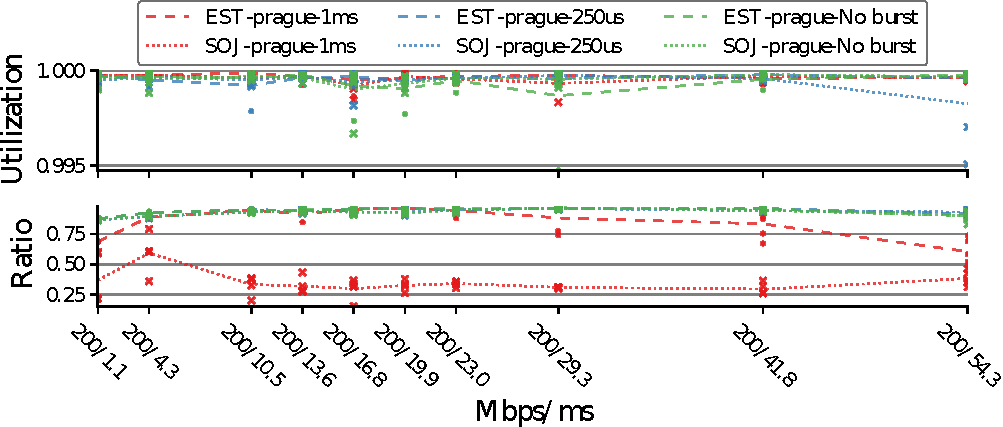
\includegraphics[width=0.85\linewidth]{experimental-AQM-root_rtt_v_util-q-ratio-prague-EST-v-SOJ-bursts1ms250us0}
	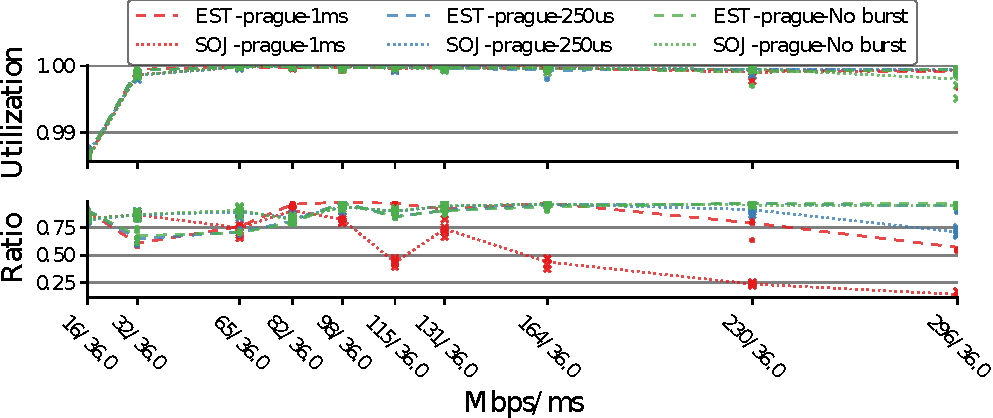
\includegraphics[width=0.85\linewidth]{experimental-AQM-root_rate_v_util-q-ratio-prague-EST-v-SOJ-bursts1ms250us0}
	\caption{TBA}\label{fig:late-comer-ratio-sweep}
\end{figure*}

\bob{Text describing experiments and commentary on results.}
\bob{Point to marking fairness appendix.}


\subsection{What Marking would be Fair?}\label{sec:marking_fairness_definition}

As remarked in \S\,\ref{sec:fairer_marking} it is obvious when marking is extremely unfair. For instance, if a bursty flow is using fraction \(\lambda\) of the capacity on average, but attracting less than fraction \(\lambda\) of the marking. However, it is not obvious how much more marking it would be fair to apply to a flow for bursts of a particular size relative to those of another flow.

The doctoral research of Wischik~\cite{Wischik99:Mark_Fairly, Wischik99:Large_Dev_PhD} and sample path shadow pricing~\cite{Kelly98:Shadow_prices_prop_fair} on which it is based appear to be the only work to tackle the question of how to define fair marking for anything but smooth flows. Wischik considers a number of possible definitions of fair marking, which is reduced down to the following three candidates, all of which are intended for offline analysis only, and infeasible for a live marking algorithm. Also all are defined in relation to packet loss, and all assume high statistical multiplexing of flows at a resource:
\begin{description}
	\item[Effective bandwidth:] EB was developed in the context of flow admission control. The EB of a variable rate flow is somewhere between its mean and peak throughputs. A bursty flow can be replaced by another flow with the same effective bandwidth without altering the resulting loss probability, including replacement by a flow with constant throughput equal to the effective bandwidth. So it would be fair to mark flows in proportion to their effective bandwidths.
	\item[\boldmath\(\Delta{L}\):] The function \(L(Y)\) is defined as the volume of loss at a resource when presented with load \(Y\). Then \(\Delta{L(Y)}\) is the change in the loss volume when the flow under consideration is removed, which is the standard definition of a shadow price, so should provide the basis for fair marking. 
	\item[Sample Path Shadow Pricing:] SPSP (\autoref{fig:spsp}) marks every packet that, if removed, would have resulted in one less packet being dropped.
\end{description}

\begin{figure}[h]
	\centering
	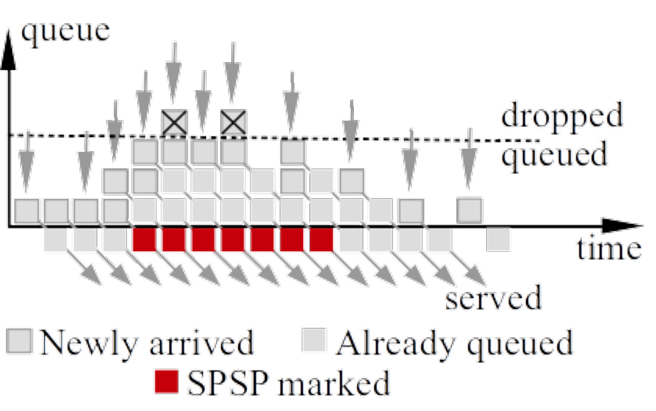
\includegraphics[width=0.8\columnwidth]{spsp}
	\caption{Schematic of Sample Path Shadow Pricing (SPSP) with one timeslot per equisized packet for illustration. A packet is marked (in red) if removing it would have resulted in one less packet being dropped}\label{fig:spsp}
\end{figure}

Wischik explains that each definition has aspects in common with the others, but they differ in their goals, assumptions and user models. 

\(\Delta{L}\) suffers from not being `incrementally fair'. As flows are added to the load, even if they are equally bursty and of equal average throughput, the rise in the volume of loss is greater for each additional flow added. So, with a certain load, imagine that the \(\Delta{L}\) due to removing any one flow is 0.3\%, but removing two equal flows reduces loss by only 0.5\%. Then if two flows band together, and internally share the marks they get under the \(\Delta{L}\) scheme between themselves, they would get only 0.25\% marking each, thereby proving that \(\Delta{L}\) is not incrementally fair.

In contrast, SPSP is incrementally fair because it acts at the granularity of packets, and is agnostic to whether packets band together under flows or users. This also means that SPSP is concerned with precisely which packets to mark, whereas \(\Delta{L}\) only knows what proportion of marks to allocate to each flow.

Like \(\Delta{L}\), EB can only say what proportion of marks should be applied to each flow but EB only knows the relative proportions; it does not know how many marks to apply overall, although this can be remedied if an exchange rate between drops and marks is defined. 

Thus, in the words of Wischik, ``SPSP is best''. However, like all the schemes, SPSP can only be applied offline---in retrospect. In the case of SPSP, this is because it is meant to mark the packets that were in the queue as it built up to the point of overflow, but many of those packets will already have left the queue by the time the queue does overflow (for instance the first four marked packets in \autoref{fig:spsp}).

Nonetheless, SPSP represents an ideal scheme that a practical marking algorithm
ought to aspire to. %Wischik proposes a marking algorithm that does just that.
% It is called Reach Overload, Send ECN (ROSE) and works as follows. Whenever
% the queue size exceeds a threshold, mark all packets in the queue. The
% threshold, \(b\), is adaptively determined as follows: for every packet that
% would have been marked by SPSP, decrease \(b\) by \(\kappa\epsilon\). For
% every packet that is marked, increase \(b\) by \(\epsilon\) \(\epsilon\) is a
% small fixed quantity and \(\kappa\) represents the number of marks that are
% equivalent to a drop, which Wischik recommends should be somewhat greater than
% one for robustness.
However, the goals of the present work are wider than those in Wischik. We particularly want to maintain very low queuing delay, but we do also want to ensure marking is as fair as possible. Therefore, it will be worth taking note of the two questions that Wischik poses to assess the fairness of a marking algorithm:
\begin{enumerate}[nosep]
	\item Does it marks packets that caused overflow, or does it mark innocent packets that arrived later?
	\item Does it mark in the busy period leading up to the overflow?
\end{enumerate}
\begin{figure}[h]
	\centering
	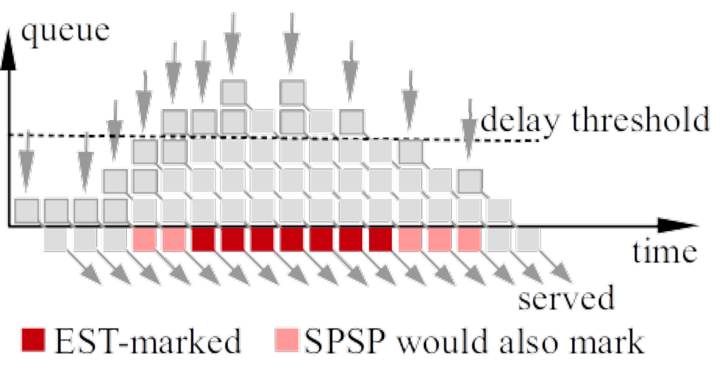
\includegraphics[width=0.9\columnwidth]{est-spsp}
	\caption{Marking based on Expected Service Time compared against Sample Path Shadow Pricing}\label{fig:est-spsp}
\end{figure}
For marking based on expected service time (EST), we redefine overflow as exceeding the queuing delay target (in time units not bytes). Then, using the example scenario in \autoref{fig:est-spsp}, we can answer the questions and justify where EST diverges. 

\begin{enumerate}[nosep, label=Q\arabic*.]
	\item EST does not mark any innocent packets; however it does not mark the packets that contributed to excess delay but were dequeued after excess delay had ended (the pink packets to the right of the red ECN-marked packets). 
	\item EST marks as many packets in the busy period leading up to excess delay as possible, but it cannot mark those that had already been served when excess delay was first detected (the pink packets to the left).
\end{enumerate}
From the earlier analysis of EST-based marking of traffic bursts (\S\,\ref{sec:marking_fairness_expts_est}), it can be seen that EST will rarely miss any packets in the build-up to excess delay, because most of the packets of a burst are still queued when the tail arrives.\footnote{Where the difference between the burst rate and the service rate of the queue is less pronounced, this would not be true. However, in the earlier analysis, bursts were always assumed to arrive in one timeslot.} Also stopping EST marking as soon as the excess delay has gone away seems preferable for two reasons:
\begin{itemize}
	\item It seems less likely to hit smoother flows, which tend to back up behind a burst, as explained in \S\,\ref{sec:fairer_marking};
	\item When there has been a period of marking, the load arriving from sources will reduce a round trip later. Thus if marking were to continue until the queue was empty, it would tend to cause under-utilization in the following round trip.
\end{itemize}

\subsection{Queue Protection and Marking Fairness}\label{sec:qprot_marking_fairness}

To end the section, \S\,\ref{sec:qprot_marking_fairness} discusses the necessity of fair marking if queue protection\footnote{aka.\ burst policing or latency policing} is to depend on it, and considers whether EST-based marking acts rapidly enough to be used as the basis of a queue protection function that can identify and remove bursts from an aggregate without identifying individual application flows.

\bob{Stitch on the above para.}

The goal of queue protection (QProt) is to try to eliminate bursty traffic from a shared low latency queue. The ability of EST-based marking to focus on bursts raises the possibility of a crude form of queue protection without having to identify layer-4 flows (in contrast to per-flow QProt specified for DOCSIS~\cite{Briscoe19b:q-prot_ID}).

Here an example design for aggregate QProt is proposed, for instance as an extension to the DualQ Coupled AQM. When a packet is about to be dequeued from the L queue, if the EST of the backlog behind it exceeds the maximum ECN-marking threshold\footnote{The step threshold, or the top of a ramp function.} by some margin, the head packet would be redirected to the back of the C queue.\footnote{Preferably by rearranging pointers, rather than moving the packet data.} The margin might be set, for instance, at twice the depth of the maximum marking threshold, or it might be slightly randomized to discouraging sources from `flying just under the radar'. Once redirection had started, it would continue until the EST at least reduced below the allowed margin, or preferably it could continue until the EST had been brought down to the maximum ECN marking threshold. 

Then, any large bursts would be more likely to be ejected from the L queue, while traffic keeping within the maximum ECN threshold would be more likely to remain in the L queue, without having to sit behind large bursts. Of course there is no guarantee that smooth traffic would not sometimes be redirected, when it happened to arrive in front of a burst. But smooth, well-behaved traffic should never build up behind a burst that had been large enough to be ejected from the L queue.

This technique would cause reordering of any flow it redirected, However, any application receiving data in bursts should not be particularly sensitive to reordering within the bursts, given one assumes it would have to buffer the bursts as they arrive anyway. Nonetheless, any even slight harm due to reordering would help to disincentivize an application from sending in bursts.

If all the traffic was bursty, perhaps because it had passed through a bursty link upstream, aggregated QProt would redirect some traffic from all flows into the C queue, which would just add reordering to all traffic. Per-flow QProt is designed to redirect the most bursty flows until queue delay reduces, so it would not necessarily fare much better in a scenario where burstiness was added to all traffic in the aggregate. However, QProt attempts to focus redirection on only a few flows, even if they are only slightly worse than others, which might help in this case. In practice, most flows would be responsive to congestion signalling so, as long as the marking was fair, aggregate burstiness should result in general under-utilization, rather than endemic reordering.\footnote{Where the IETF draft on L4S~\cite{Briscoe15f:ecn-l4s-id_ID} discusses burstiness from upstream links, it suggests that the pragmatic solution is to improve the configuration of the system as a whole, for instance reducing the burstiness of an upstream link, or increasing the L4S marking threshold at the bottleneck.}

The above aggregate QProt technique is not necessarily only applicable to a DualQ. It is simple enough that it could potentially also be included in a per-flow queue, to protect against the possibility of a bursty flow encapsulated within a VPN alongside smooth flows. For instance, the L4S architecture allows for the possibility that VPNs are separated into two sister per-flow queues for L4S and non-L4S packets. Then the L4S per-`flow' queue could redirect bursts into its non-L4S sister. However, a bursty flow within a VPN is perhaps a corner case that would not warrant such an addition.

% ================================================================
\section{Discussion}\label{sec:discussion}
\subsection{Distributed Queues}\label{sec:sojourn-distrib}

Using sojourn time leverages the advantage that it can be measured across a complex set of queues, including the case where the initial enqueue and the final dequeue routines are distributed across different machines or processors, as already mentioned (separate clocks would need to be synchronized).

This could include the case where the inputs are located on multiple client machines (e.g.\ mobile user equipment, WiFi stations, cable modems or passive optical network modems) while the output is a located at an aggregation node (e.g.\ a cellular base station (eNodeB)~\cite{Tan09:AQM_uplink_patent}, a WiFi access point (AP), a centralized controller for multiple WiFi APs, a cable modem terminal server (CMTS) or optical line termination (OLT) equipment), with a multiplexed access network between the clients and the aggregation node.

In complex cases like these, if minimization of measurement delay is important, the best approach to use will depend on which of metrics are most feasible to measure and communicate to the dequeue process, which will depend on the architecture of the distributed queues. \autoref{tab:distrib-qs} tabulates which metrics are needed by which approach.

\begin{table*}[h]
	\begin{center}
		\begin{tabular}{ll|cc}
			& 				& Time-based backlog & Scaled sojourn time\\
			\hline
			\multirow{2}{*}%
			{enqueue time}& arrival time		& -					& \checkmark \\
			& backlog				& -					& \checkmark \\
			\hline
			\multirow{4}{*}%
			{dequeue time}& departure time		& \checkmark		& \checkmark \\
			& backlog				& \checkmark		& \checkmark \\
			& serialization time	& \checkmark		& - \\
			& packet size			& \checkmark		& - \\
		\end{tabular}
	\end{center}
	\caption{Metrics needed by each approach}%
	\label{tab:distrib-qs}
\end{table*}

Note that the backlog at enqueue time and the backlog at dequeue time need to include all the data buffered between the two, not just that in the ingress and egress buffers. Therefore the backlog metric is probably the critical factor for feasibility. And given both approaches need the backlog at dequeue time, and scaled sojourn also needs the backlog at enqueue time, scaled sojourn might end up being the more complex approach.`

For instance, on a single machine, the \texttt{count\_enq} variable would be available in a memory shared between ingress and egress. But if the ingress and egress are separate, the ingress machine would have to communicate the \texttt{count\_enq} variable to the egress over a (preferably non-blocking) control channel, so that the egress could calculate \texttt{backlog\_deq} by subtracting \texttt{count\_deq}. 

Certain access network technologies, e.g.\ those for cellular radio access networks, already include such a control channel, over which buffer status report (BSR) control messages are sent from the user equipment to the radio network controller. The delay to access a control variable at the input machine from the output machine would be larger than that in a non-distributed system, but it would at least be a known, constant delay. So the control system could still provide robust metrics to control queuing in the data channel.

As well as the aggregation node using expected service time (EST) to apply congestion signalling within the final dequeue routine (effectively on behalf of the input queue), the aggregation node could also use EST to govern the scheduling algorithm for controlling each client's inward (upstream) access rate into the shared medium, by altering the rate at which it granted medium access slots to each client.

\subsection{Applicability of Expected Service Time}\label{sec:inst_svc_time_applic}

Using any of the approaches in \S\,\ref{sec:exp_svc_time} to calculate EST would improve timeliness relative to using sojourn time or other techniques to measure queue delay. However, it would not be worth modifying an existing deployment unless all other delays were going to be removed at the same time. 

It might be thought that an algorithm like the proportional integral (PI) controller\footnote{Used in QCN~\cite{IEEE802.1Qau:Ethernet_QCN}, PIE~\cite{Pan17:PIE}, PI2~\cite{DeSchepper16a:PI2} or the base AQM of DualPI2~\cite{Briscoe15e:DualQ-Coupled-AQM_ID}.} already takes account of the change in queuing delay between samples, so changing the queuing delay measurement itself seems redundant. However, using EST actually ensures that a PI algorithm takes account of the change between the latest queue delay measurements at each sample time, not between two outdated measurements.

It might also be thought that PI controllers do not need to care so much about instantaneous measurements, because they are maintaining the fairly large queue that is needed by classic congestion control algorithms like Reno, Cubic, Compound or BBRv1. However, even though a PI algorithm only samples the queue fairly infrequently (relative to packet serialization time), using an out of date queue metric makes it necessary to introduce extra heuristic code to deal with the resulting sloppiness.

For instance, in the case of PIE~\cite{Pan17:PIE}, some heuristic code suppresses any drop once the last sample of queue delay falls below half the target delay.\footnote{As long as some other conditions hold that are not important here.} This is an attempt to suppress drop when the queue is draining after the load has gone idle. However, it is ineffective if sojourn time is used to measure the queue, because the sojourn time does not reduce until after the last packet (as explained in \autoref{fig:sojourn-prob}b). Using EST whenever queue delay is sampled should eliminate the need for this heuristic because it takes account of the reducing backlog as the queue drains.\footnote{Indeed, this was the original motivation for this work.}

EST is also applicable to the CoDel algorithm for the same reasons---sojourn time fails to take account of the evolution of the queue after the head packet was enqueued (again, as in \autoref{fig:sojourn-prob}b). This can tend to cause the AQM to continue dropping or marking packets at the end of a flow, because the sojourn time does not recognize that the queue has gone below the target delay. The CoDel code in Linux includes a heuristic to exit dropping mode when the backlog goes below 1\,MTU, but that still continues dropping mode until the last packets of a flow, and tail loss is particularly problematic for a flow to detect.

EST is particularly applicable to a simple AQM algorithm like the time-based shallow threshold recommended for DCTCP in~\cite{Bai16:MQ-ECN} or the native AQM for L4S traffic in DualPI2~\cite[Appx.\ A]{Briscoe15e:DualQ-Coupled-AQM_ID} or Low Latency DOCSIS~\cite{CableLabs:DOCSIS3.1}\footnote{Although in the case of DOCSIS, it is hard to manipulate the ECN field at the head of the queue, because a pipeline of processes has already been set in motion.}. It would be applicable whether the threshold is a simple step, or a probabilistic ramp like the RED function (but based on instantaneous queue delay, not smoothed queue length), or a deterministic ramp or convex function of instantaneous queueing delay, as in Curvy RED~\cite[Appx.\ B]{Briscoe15e:DualQ-Coupled-AQM_ID}. The queue in these cases is intended to be very shallow, so it might seem that the extra measurement delay would be minimal. However, the sensitivity of these very low delay schemes to burstiness makes it particularly important to ensure that bursts are measured rapidly and correctly.

EST could apply to many types of queue, not just packet queues, as long as the size of each job is quantified in common units that are additive. Examples include, but are not limited to, queues of datagrams, frames or packets, as well as message queues, call-server queues, computer process scheduling queues, storage queues (e.g. SSD or disk), workflow queues for mechanical or human-operated stages of tasks. 

As well as dropping or ECN-marking, different sanctions could be applied using the same basic ideas. Examples include, but are not limited to: truncating or otherwise damaging the data or checksum of a message or packet but preserving the information necessary for delivery; rerouting; delaying; downgrading the class of service; and tagging.

% ================================================================
\section{Other Signalling Delays}\label{sec:other_delays}

The introduction enumerated six causes of delay to congestion signals and highlighted two that this memo would focus on. The other four sources of signalling delay are briefly surveyed below, with pointers to where they have been considered in other work.

\subsection{Propagation Delay} Numerous proposals have been made to speed up signalling by sending the signal from the queue back against the flow of traffic, direct to the sender. This can be done in a pure L2 network, e.g. backwards congestion notification (BCN) in IEEE 802.1Qau~\cite{IEEE802.1Qau:Ethernet_QCN} a.k.a.\ Quantized Congestion Notification (QCN), which is now rolled into 802.1Q-2011 and 802.1Q-2014. However, in general signalling backwards is problematic in IP networks, amongst other reasons because the sender has to accept out-of-band packets from any arbitrary source in the middle of the network, which makes it vulnerable to DoS attacks~\cite{IETF_RFC6633:ICMP_SQ_Depr}. 

Therefore, here we will assume that signals are piggy-backed on the forward traffic flow then fed back to the sender via the receiver. However, this does not preclude a solution to the problems of backwards congestion notification.

\subsection{Smoothing Delay} AQMs designed for the Internet's classic congestion controls (TCP Reno, Cubic, Compound, etc.) filter out fluctuations in the queue by smoothing it before using the smoothed measurement as a measure of load to drive the congestion signal. DCTCP~\cite{Alizadeh10:DCTCP} proposed to smooth the signal at the sender, so that the network could send out the signal immediately, without smoothing, and L4S followed this approach~\cite{Briscoe16a:l4s-arch_ID}. This allows the sender to receive the signal without smoothing delay, which is particularly useful in cases where the sender might not need to smooth the signal itself, e.g.\ to detect overshoot when accelerating to start a new flow. Shifting the smoothing function from the network to the sender also makes sense because the network does not know the round trip time (RTT) of each flow, so it has to smooth over the maximum likely RTT. Whereas a sender knows its own RTT and can smooth over this timescale.

\subsection{Signal encoding delay} Previous research has proposed to change the IP wire protocol to provide more bits to signal congestion. Nonetheless, it has been pointed out\footnote{Matt Mathis is believed to have pointed this out first.} that the delay of a unary encoding is inversely proportional to the value being encoded, and the congestion window of a scalable congestion control is also inversely proportional to the value of the congestion signal. So, as flow rates (and consequently congestion windows) increase over the years, at least in general the delay to encode the signal does not increase.\footnote{However, encoding delay does increase with the degree of ACK coalescing.}

Therefore, in this report we have assumed the unary encoding of congestion signals standardized as ECN by the IETF~\cite{IETF_RFC3168:ECN_IP_TCP}. This does not preclude other encodings, e.g. the multi-bit encoding of QCN or minor alterations to the decoding to avoid saturation, such as that in \cite{Briscoe17a:CC_Tensions_TR}.

\subsection{Removing Randomness Delays}\label{sec:rand_delay}

One of the main motivations for the design of Random Early Detection (RED)~\cite{Floyd93:RED} was to break up synchronization between the sawteeth of TCP flows driving the same queue. This still remains an important requirement for all AQM algorithms~\cite{Baker15:AQM_Recommendations}.

AQMs mitigate synchronization by introducing marking or dropping more gradually than a tail-drop buffer would, and to a certain extent by randomizing the marking. 

With clean-slate approaches such as DCTCP in private networks, or incrementally deployable clean-slate approaches like L4S~\cite{Briscoe16a:l4s-arch_ID} for the public Internet, requirements for the network and for end-systems are still in the process of definition. In these clean-slate or slightly dirty-slate cases, it would be possible to require the sender's congestion control to dither its response to congestion signals, so that it would not be necessary to introduce randomness in the network, which adds uncertainty and therefore delay to the congestion signalling channel. 

Any AQM that probabilistically signals congestion with probability \(p\) could deterministically signal congestion by introducing an interval of \(1/p\) packets between each drop or mark. PDPC+~\cite{Sagfors03:PDPC_vary} and CoDel~\cite{Nichols12:CoDel}, which is very similar, use a deterministic rather the probabilistic algorithm to encode the congestion signal. Both AQMs in DualPI2~\cite[Appx.\ A]{Briscoe15e:DualQ-Coupled-AQM_ID} also uses a deterministic algorithm.

The determinism would be lost wherever the AQM was controlling flows multiplexed within one queue without per-flow state, because assignment of each deterministic congestion signal to each flow would become randomized by even slightly random packet arrivals from the different flows~\cite{Briscoe15d:PIE_rvw}.

Nonetheless, whenever a flow is on its own in an AQM, which is a common case for the traffic patterns in many access network designs,  deterministic congestion signalling would reduce signalling delay. This could particularly ease the design of new flow-start algorithms, where the flow introduces microbursts or chirps to sense at what level it starts to congest the link.

Determinism of an AQM is of less importance when the congestion control rather than the AQM determines the spacing between marks. For instance, the duration of the sawteeth of a classical congestion control scales with BDP. So at low BDP, the AQM determines the spacing between marks, but as BDP scales, the congestion control sawteeth move in and out of closed loop control, which determines the duration between `congestion events' with the AQM inactive between times~\cite[\S\,3.3]{Briscoe21c:pi2param}.